\documentclass[10pt,a4j,twoside]{jarticle}
\usepackage{amsmath}
%\usepackage{mathabx}
%\usepackage{psfig}
\usepackage{graphicx} % use \includegrahpics
%\usepackage{Tabular}

\usepackage{enumsty}

\def\figref#1{図~\ref{#1}}
\def\tabref#1{表~\ref{#1}}
\def\eqref#1{(\ref{#1})~式}
\def\eqrefbare#1{\ref{#1}}
\def\secref#1{\ref{#1}~節}
\def\Theoref#1{定理~\ref{#1}}
\def\Lemref#1{補題~\ref{#1}}

\pagestyle{bothstyle}
\makeatletter
%\def\@oddfoot{\hbox to \textwidth{\fhil \thepage \hfil}}
%\def\@oddfoot{\reset@font\hfil\thepage\hfil}%
\makeatother

\makeatletter
\@addtoreset{equation}{section}
\renewcommand{\theequation}{\thesection.\@arabic\c@equation}
\makeatother

%\usepackage{showlabel}

%%----------------------------------------------------------------------
%%
\usepackage{bm}
%\def\V#1{\mbox{\boldmath $#1$}}
%\def\M#1{\mbox{\boldmath $#1$}}
%\def\S#1{\mbox{\boldmath $#1$}}
%\def\Ts#1{\mbox{\boldmath $#1$}}
\def\V#1{{\bm{#1}}}
\def\M#1{{\bm{#1} }}
\def\S#1{{\bm{#1}}}
\def\Ts#1{{\bm{#1}}}

\usepackage{amsmath}
\usepackage{amssymb}
\usepackage{amsfonts}

\def\SetNat{\mathbb{N}}  % 自然数集合
\def\SetInt{\mathbb{Z}}  % 整数集合
\def\SetRat{\mathbb{Q}}  % 有理数集合
\def\SetReal{\mathbb{R}} % 実数集合
\def\SetComp{\mathbb{C}} % 複素数集合

\def\Deg#1{^{\left< #1 \right>}}  % 次数
\def\Cxc#1{{#1}^{\dagger}} % 複素共役

\def\Abs#1{\left| #1 \right|}

\def\MtxK#1#2{\left[ \begin{array}[c]{#1} #2 \end{array} \right]}
\def\Vec#1{\MtxK{c}{#1}}
\def\Mtxxxx#1{\MtxK{cccc}{#1}}
\def\Mtxx#1{\MtxK{cc}{#1}}
\def\Mtx#1{\MtxK{c}{#1}}
\def\Tsr#1{\MtxK{c}{#1}}

\def\Dpd{\times} %% 直積記号 : direct product
\def\Kpd{\otimes} %% クロネッカー積記号 : Kronecker product
\def\DpA#1{\bar{#1}}  %% 直積の値の頭につけるアクセント

\def\MxA#1{\hat{#1}}  %%  混合分布につけるアクセント

\def\Est#1{\hat{#1}}    %% estimate
\def\Apx#1{\tilde{#1}}  %% approx

\def\Av#1{\left|#1\right|}
\def\SD#1{\sigma_{#1}}
\def\Var#1{\SD{#1}^2}
\def\Avg#1{\mu_{#1}}
\def\Xpt#1{\bar{#1}}  %% 期待値

\def\Seq#1{\left\{ #1 \right\}}
\def\Set#1{\left\{ #1 \right\}}
\def\Tuple#1{\left< #1 \right>}

\makeatletter
  \def\@LkS{{\cal L}}    %% likelihood Symbol
  \def\@LkF[#1]{\@LkS\left(#1\right)}    %% likelihood func.
  \def\Lk{\@ifnextchar[{\@LkF}{\@LkS}% ]
         }
\makeatother

\makeatletter
  \def\@PrSym{{\cal P}}
  \def\Pr{\@ifnextchar[{\@Pr}{\@PrSym}% ]
  }
  \def\@Pr[#1]{\@PrSym\left(#1\right)}

  %% Gaussian  G[x;\mu,\sigma]
  \def\@GSym{{\cal G}}        
  \def\G{\@ifnextchar[{\@G}{\@GSym}% ]
  }
  \def\@G[#1]{\@GSym\left(#1\right)}

%% 二項分布・Binomial 
  \def\@BnSym{{\cal B}}
  \def\Bn{\@ifnextchar[{\@Bn}{\@BnSym}% ]
  }
  \def\@Bn[#1]{\@BnSym\left(#1\right)}

%% 幾何分布・geometric distribution
  \def\@GmSym{\mathsf{g}}
  \def\Gm{\@ifnextchar[{\@Gm}{\@GmSym}% ]
  }
  \def\@Gm[#1]{\@GmSym\left(#1\right)}

%% noise
  \def\nz{\epsilon}	


\makeatother


\def\EqDesc#1{\mbox{\ \ \ ; #1}}


\makeatletter
\def\Lp{\@ifnextchar[{\@Lp}{{\cal L}}} %% ラプラス変換 \Lp[f] or \Lp(f)
\def\@Lp[#1]{\Lp{}\left[#1\right]}
\def\ILp{\@ifnextchar[{\@ILp}{{\cal L}^{-1}}} %% ラプラス変換 \Lp[f] or \Lp(f)
\def\@ILp[#1]{\ILp{}\left[#1\right]}
\makeatother

\def\Conv{\ast}  %% 畳み込み積分 (Convolution Integral)
\def\Comb#1#2{{}_{#1}C_{#2}}

%%======================================================================

\def\Where{\mbox{\hspace{3em}} ; \mbox{\hspace{1em}}}
\def\where0pt{\makebox[0pt][l]{\mbox{where}} \nonumber}


\def\MyBox#1{{\unitlength=#1 \framebox(1,1){}}}
\def\MyFillBox#1{\rule{#1}{#1}}
\def\EOTH{\hfill\MyBox{.5em}}
\def\QED{\hfill\MyFillBox{.5em}}

\newenvironment{Note}[1]{%
%  \paragraph*{ノート: #1} \fill \rule{0.5\textwidth}{1pt}
  \paragraph{\protect\MyFillBox{1em} ノート--- #1} \hrule%
  \hfill 
}{%
  \hfill\MyBox{1em}\hrule
  \ \\
}

%%======================================================================

\newif\ifWideBoxedEqnarray
\WideBoxedEqnarraytrue
\WideBoxedEqnarrayfalse

\newenvironment{BoxedEqnarray}{%
  \vspace{-4ex}
  \begin{center}%
    \begin{tabular}[c]{|c|} \hline%
      \begin{minipage}[c]{\textwidth}  %{width}
      \ifWideBoxedEqnarray%
        \vspace{-0.5ex} %
      \else%
        \vspace{-2.3ex} %
      \fi%
        \begin{eqnarray}%
}{%
        \end{eqnarray}%
      \end{minipage}%
      \ifWideBoxedEqnarray%
        \\%
      \else%
        % nothing
      \fi%
%      \\
      \\ \hline%
    \end{tabular}
  \end{center}%
}

%%======================================================================

\def\DefPrefix{定義}
\def\LemmaPrefix{補題}
\def\TheoremPrefix{定理}
\newtheorem{genericTheorems}{GenericTheorem}[section]
\newtheorem{xDef}[genericTheorems]{\DefPrefix}
\newtheorem{xLemma}[genericTheorems]{\LemmaPrefix}
\newtheorem{xTheorem}[genericTheorems]{\TheoremPrefix}

\newenvironment{Lemma}{%
  \begin{xLemma}%
    \addcontentsline{toc}{subparagraph}{%
      \fbox{\LemmaPrefix \thexLemma}}
  \ \\
}{%
  \EOTH%
  \end{xLemma}%
}

\newenvironment{Theorem}{%
  \begin{xTheorem}%
    \addcontentsline{toc}{subparagraph}{%
      \fbox{\TheoremPrefix \thexLemma}}
  \ \\
}{%
  \EOTH
  \end{xTheorem}%
}


\newenvironment{Proof}{%
  \paragraph*{証明}%
  \vrule width .7\linewidth height 0.01pt
  \ \par%
}{%
  \\
  \vrule width .7\linewidth height 0.01pt
  \QED%
}





%\iftrue
\iffalse
\includeonly{
  S010/secBody.primePair
  }
\fi

%\def\ClearPage{\clearpage}
\def\ClearPage{\cleardoublepage}

\begin{document}
%%----------------------------------------------------------------------
\title{IS Lab. 問題集}
\author{野田五十樹}
\date{%
  {\scriptsize
  \begin{tabular}[c]{|l|l|} \hline
  2024/02/23 & 素数組問題 \\ \hline
  2024/02/23 & 階乗問題 \\ \hline
  2024/02/23 & お釣り問題 \\ \hline
  2024/02/23 & 複素数問題 \\ \hline
 \end{tabular}
  }
}
\maketitle
%%----------------------------------------------------------------------

\setcounter{tocdepth}{10}

\iftrue
%\iffalse
\ClearPage
\tableofcontents
\ClearPage\cleardoublepage
\fi

%%----------------------------------------------------------------------
\section{素数の組}
\label{s:素数の組}
%% - - - - - - - - - - - - - - - - - - - - - - - - - - - - - - - - - - -

%%--------------------------------------------------
\subsection{問題}
\label{ssec:素数の組:問題}
%% - - - - - - - - - - - - - - - - - - - - - - - - -

$p^q + q^p$ が素数になる素数の組 $\Tuple{p,q}$ を全て求めよ。
ただし、$p<q$ とする。

\clearpage
%%--------------------------------------------------
\subsection{解答}
\label{ssec:素数の組:解答}
%% - - - - - - - - - - - - - - - - - - - - - - - - -

$p,q$ が共に奇数の素数とする。
その場合、$p^q, q^p$ は共に2より大きい奇数となる。
よって、$p^q + q^p$ は2より大きい偶数になり、素数ではない。

よって、$p,q$ はいずれかは偶数の素数、すなわち $2$ となる。
また、$p < q$ から、$p = 2$ となる。

$q = 3$ の場合、$p^q + q^p = 2^3 + 3^2 = 8 + 9 = 17$ となり、素数である。
よって、 $\Tuple{2,3}$ は条件を満たす組となる。

$q > 3$ の場合、
2の倍数、3の倍数は素数ではないので、
$q = 6k \pm 1$ と表される。
よって、
  %%$$$$$$$$$$$$$$$$$$$$$$$$$$$$$$$$$$$$$$$$$$$$$$$$$$$$$$$$$$$$$$$$$$$$$$
  \begin{eqnarray}
    p^q + q^p
      & = &
        2^{6 k \pm 1} + (6 k \pm 1)^2
  \\
      & = &
        2 + 1   \mod 3
  \\
      & = &
        3
  \\
      & = &
        0   \mod 3
  \end{eqnarray}
  %%$$$$$$$$$$$$$$$$$$$$$$$$$$$$$$$$$$$$$$$$$$$$$$$$$$$$$$$$$$$$$$$$$$$$$$
となり、かならず 3 で割り切れる。
すなわち、素数ではない。

よって、$q > 3$ の場合、条件を満たす組 $\Tuple{p,q}$ は存在しない。

よって、条件を満たす素数の組は、$\Tuple{2,3}$ のみである。
\QED






\ClearPage\cleardoublepage
%%----------------------------------------------------------------------
\section{階乗に関する問題}
\label{s:階乗}
%% - - - - - - - - - - - - - - - - - - - - - - - - - - - - - - - - - - -

%%--------------------------------------------------
\subsection{階乗を割った余り}
\label{ssec:階乗:階乗を割った余り}
%% - - - - - - - - - - - - - - - - - - - - - - - - -
%%-----------------------------
\subsubsection{問題}
\label{sssec:階乗:階乗を割った余り:問題}
%% - - - - - - - - - - - - - -

$100 !$ を $97$ で割った余りはいくらか?


\clearpage
%%------------------------------
\subsubsection{解答}
\label{sssec:階乗:階乗を割った余り:解答}
%% - - - - - - - - - - - - - - -

$100 ! = 100 \cdot 99 \cdot 98 \cdot 97 \cdot 96 \ldots$ であるので、
$100!$ は $97$ を因子として持つ。
よって、$100!$ を $97$ で割った余りは 0 である。


%%------------------------------
\subsubsection{参考: Wilson の定理}
\label{sssec:階乗:階乗を割った余り:参考}
%% - - - - - - - - - - - - - - -

\begin{Theorem}
  $p$ が素数ならば、 $(p-1)! = -1 \mod p$ である。
  \\
  逆に、自然数 $p > 1$ に対し $(p-1)! = -1 \mod p$ ならば、
  $p$ は素数である。
\end{Theorem}
  

\clearpage
%%--------------------------------------------------
\subsection{階乗の階乗を割った余り}
\label{ssec:階乗:階乗の階乗を割った余り}
%% - - - - - - - - - - - - - - - - - - - - - - - - -

%%-----------------------------
\subsubsection{問題}
\label{sssec:階乗:階乗の階乗を割った余り:問題}
%% - - - - - - - - - - - - - -

$(100 !)!$ を $(99!)^{100}$ で割った余りはいくらか?


\clearpage
%%------------------------------
\subsubsection{解答}
\label{sssec:階乗:階乗の階乗を割った余り:解答}
%% - - - - - - - - - - - - - - -

\begin{Lemma}
  自然数$n,m$ で、$n \ge m$ の時、
  $n!$ は $m! \cdot (n-m)!$ で割り切れる。
\end{Lemma}

\begin{Theorem}
  自然数の列 $\Seq{k_1, k_2, \cdots, k_n}$ を考える、この時、
  $\left( \sum_{i=1}^{n} k_i \right) !$ は
  $\prod_{i=1}^{n} k_i !$ で割り切れる。
\end{Theorem}

$k_1 = k_2 = \cdots = k_{100!} = 99!$ とすれば、
$\sum_{i=1}^{100} k_i = 100 \cdot 99! = 100!$ であり、
$\prod_{i=1}^{100} k_i = (99!)^{100} $ である。
これにより、上記の定理を使うと、
$(100!)!$ は $(99!)^{100}$ で割り切れる。
\QED





\ClearPage\cleardoublepage
%%----------------------------------------------------------------------
\section{お釣りが足りている}
\label{s:お釣り}
%% - - - - - - - - - - - - - - - - - - - - - - - - - - - - - - - - - - -

%%--------------------------------------------------
\subsection{問題}
\label{ssec:お釣り:問題}
%% - - - - - - - - - - - - - - - - - - - - - - - - -

%%--------------------------------------------------
\subsubsection{具体的問題}
\label{sssec:お釣り:問題:具体的問題}
%% - - - - - - - - - - - - - - - - - - - - - - - - -

ある商人が1個50円のおもちゃを10個売っているとする。
お客は、各々1つずつそのおもちゃを買うとし、
支払いには、100円玉か50円玉でしか支払わないとする。
商人は、最初、お釣り用の50円玉を4枚用意しているとする。
おもちゃ10個が売り切れた時、
商人の手元には50円玉が2枚あった。

この場合、お客が支払った50円玉・100円玉の順序の場合の数は何通りあるか?

%%--------------------------------------------------
\subsubsection{一般化問題}
\label{sssec:お釣り:問題:一般化問題}
%% - - - - - - - - - - - - - - - - - - - - - - - - -

\secref{sssec:お釣り:問題:具体的問題}の問題で、おもちゃの数を $n$ 個、
最初に用意した50円玉の枚数を $m$ 枚、
最後の残った50円玉の枚数を $l$ 枚とした時、
お客が支払った50円玉・100円玉の順序の場合の数は何通りあるか?


%%--------------------------------------------------
\subsubsection{派生系具体的問題}
\label{sssec:お釣り:問題:派生系具体的問題}
%% - - - - - - - - - - - - - - - - - - - - - - - - -

以下のようなカッコばかりの文字列を考える。
\begin{quote}
  \verb|(((((__________)))|
\end{quote}
文字列の構成は、まず先頭に開きカッコ ``('' が5個並び、
続いて空白 ``\verb|_|'' が10個並び、
最後に閉じカッコ ``)'' が3つ並んでいる。
この空白の部分に開きカッコと閉じカッコを合計10個入れ、
最終的に、この文字列の最後の閉じカッコでちょうど
先頭の開きカッコが閉じられるようにしたい。
空白に並べるカッコの順列組み合わせはいくつか?

ただし、文字列の途中で最初のカッコが閉じられではいけない。

%%--------------------------------------------------
\subsubsection{派生系一般化問題}
\label{sssec:お釣り:問題:派生系一般化問題}
%% - - - - - - - - - - - - - - - - - - - - - - - - -

\secref{sssec:お釣り:問題:派生系具体的問題}の問題で、
空白の数を $n$ 個、
最初の開きカッコの数を $m$ 個
最後の閉じカッコの数を $l$ 個とした時、
空白に並べるカッコの順列組み合わせはいくつか?


\clearpage
%%--------------------------------------------------
\subsection{解答}
\label{ssec:お釣り:解答}
%% - - - - - - - - - - - - - - - - - - - - - - - - -

%%--------------------------------------------------
\subsubsection{具体的問題}
\label{sssec:お釣り:解答:具体的問題}
%% - - - - - - - - - - - - - - - - - - - - - - - - -

問題の設定により、
おもちゃが1つ売れる毎に50円玉は1枚増えるか1枚減るかたちで
枚数が変化する。

その様子を表したのが、\figref{fig:S030/Figs/Figure.change.p01}である。
横軸は売れたおもちゃの数、
縦軸が50円玉の数であり、
$(0,4)$ から出発して、$(10,2)$ に至る斜めの碁盤目の経路を辿ることになる。

この内、お釣りの50円玉が足らなくなるのは、図の赤い経路を通る場合である。
つまり、\figref{fig:S030/Figs/Figure.change.p01}で示される碁盤目のうち、
赤い経路を通らない経路の数を数えれば良い。

まず、赤い経路を無視して、全ての碁盤目の経路を数え上げると、
10個の選択肢の中から順不同で4つ選ぶ場合の数であるので、
  %%$$$$$$$$$$$$$$$$$$$$$$$$$$$$$$$$$$$$$$$$$$$$$$$$$$$$$$$$$$$$$$$$$$$$$$
  \begin{eqnarray}
    N_{\text{all}} & = & _{10}C_{4}
  \\
      & = &
        \frac{10!}{4! 6!}
  \\
      & = &
        210
  \end{eqnarray}
  %%$$$$$$$$$$$$$$$$$$$$$$$$$$$$$$$$$$$$$$$$$$$$$$$$$$$$$$$$$$$$$$$$$$$$$$
  
次に、
全て数え上げた中から、お釣りが足らなかった経路を取り上げる。
この時、お釣りが足らなくなった瞬間から、
50円玉の残り数を示す碁盤目を辿る方向を反転させるとする。
すると、
その経路が行き着く先は、
\figref{fig:S030/Figs/Figure.change.p02}のように、
$y=-1$ のところで鏡像にした経路を描く。
よって、その後、$(10,2)$ にたどり着いていた経路は、
この鏡像にした経路の中では、$(10,-4)$ に辿り着く。

そこで、$(0,4)$から$(10,-4)$ に辿る経路を数え上げると、
10個の選択肢の中から1つ順不同で選び出す場合の数であるので、
  %%$$$$$$$$$$$$$$$$$$$$$$$$$$$$$$$$$$$$$$$$$$$$$$$$$$$$$$$$$$$$$$$$$$$$$$
  \begin{eqnarray}
    N_{\text{short}} & = & _{10}C_{1}
  \\
      & = &
        \frac{10!}{1! 9!}
  \\
      & = &
        10
  \end{eqnarray}
  %%$$$$$$$$$$$$$$$$$$$$$$$$$$$$$$$$$$$$$$$$$$$$$$$$$$$$$$$$$$$$$$$$$$$$$$

  %%$$$$$$$$$$$$$$$$$$$$$$$$$$$$$$$$$$$$$$$$$$$$$$$$$$$$$$$$$$$$$$$$$$$$$$
  \begin{eqnarray}
    N_{\text{ans}} & = & N_{\text{all}} - N_{\text{short}}
  \\
      & = & 210 - 10
  \\
      & = & 200
  \end{eqnarray}
  %%$$$$$$$$$$$$$$$$$$$$$$$$$$$$$$$$$$$$$$$$$$$$$$$$$$$$$$$$$$$$$$$$$$$$$$

よって答えは、200通り。


%%FFFFFFFFFFFFFFFFFFFFFFFFFFFFFFFFFFFFFFFFFFFFFFFFFFFFFFFFFFFFFFFFFFFFFF
\begin{figure}
  \begin{minipage}[c]{.49\linewidth}  %{width}
  \centering
  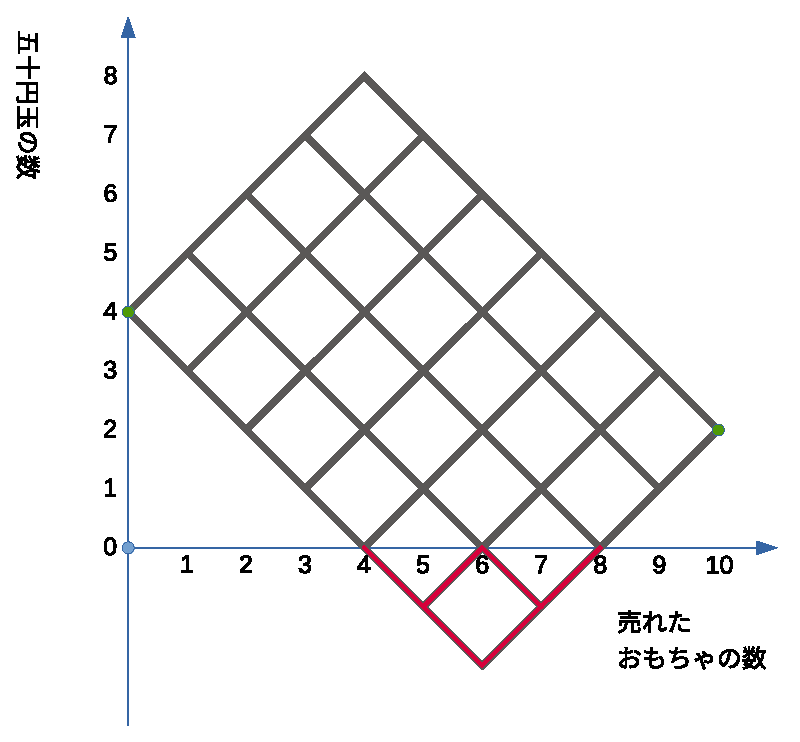
\includegraphics[width=5cm]{S030/Figs/Figure.change.p01.eps}
  \caption{お釣り玉の残数の変化経路図}
  \label{fig:S030/Figs/Figure.change.p01}
  \end{minipage}~
%\end{figure}
%%FFFFFFFFFFFFFFFFFFFFFFFFFFFFFFFFFFFFFFFFFFFFFFFFFFFFFFFFFFFFFFFFFFFFFF
%%FFFFFFFFFFFFFFFFFFFFFFFFFFFFFFFFFFFFFFFFFFFFFFFFFFFFFFFFFFFFFFFFFFFFFF
%\begin{figure}[b]
  \begin{minipage}[c]{.49\linewidth}  %{width}
  \centering
  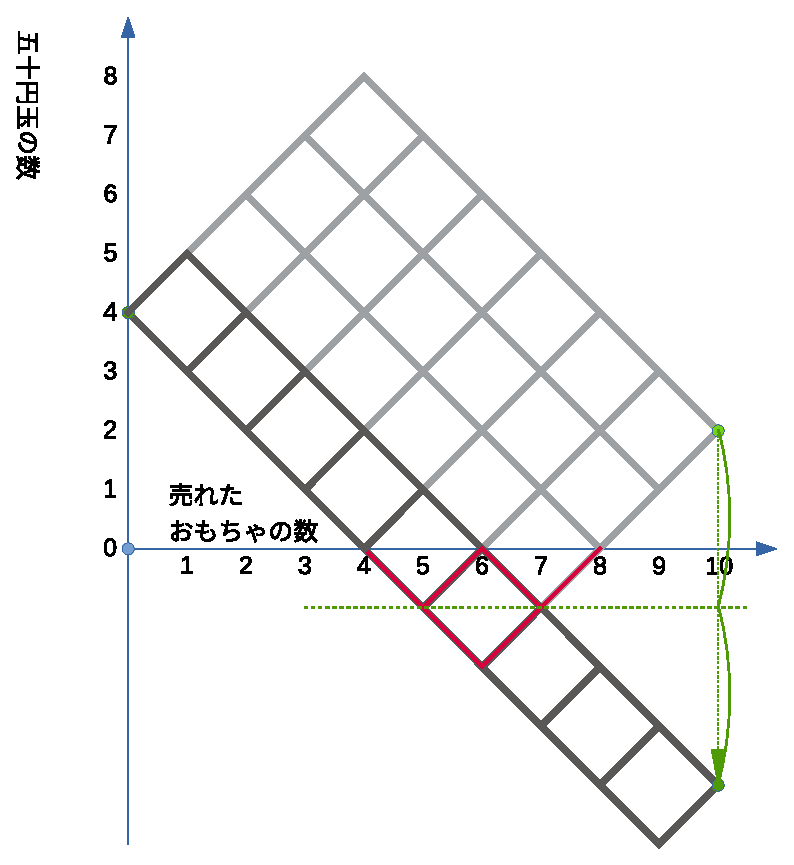
\includegraphics[width=5cm]{S030/Figs/Figure.change.p02.eps}
  \caption{お釣り玉が足らなくなる場合の残数の変化経路図}
  \label{fig:S030/Figs/Figure.change.p02}
  \end{minipage}
\end{figure}
%%FFFFFFFFFFFFFFFFFFFFFFFFFFFFFFFFFFFFFFFFFFFFFFFFFFFFFFFFFFFFFFFFFFFFFF


%%--------------------------------------------------
\subsubsection{一般化問題}
\label{sssec:お釣り:解答:一般化問題}
%% - - - - - - - - - - - - - - - - - - - - - - - - -

上記と同じ考え方をすると、
お釣りが足らなくなる場合の考えずに全ての経路を考えると、
$(0,m)$ から $(n,l)$ に至る斜めの碁盤目の経路となる。
この経路の数は
$n$ の候補の中から $\frac{n - (m-l)}{2}$ を順不同で選び出す場合の数であるので、
以下のように表せる。
  %%$$$$$$$$$$$$$$$$$$$$$$$$$$$$$$$$$$$$$$$$$$$$$$$$$$$$$$$$$$$$$$$$$$$$$$
  \begin{eqnarray}
    N_{\text{all}} & = & _{n}C_{\frac{n - (m-l)}{2}}
  \end{eqnarray}
  %%$$$$$$$$$$$$$$$$$$$$$$$$$$$$$$$$$$$$$$$$$$$$$$$$$$$$$$$$$$$$$$$$$$$$$$

一方、お釣りが足りなくなる経路の数は、
$(0,m)$ から $(n,-l-2)$ に至る斜めの碁盤目の経路となる。
この経路の数は
$n$ の候補の中から $\frac{n - (m+l+2)}{2}$ を順不同で選び出す場合の数であるので、
以下のように表せる。
  %%$$$$$$$$$$$$$$$$$$$$$$$$$$$$$$$$$$$$$$$$$$$$$$$$$$$$$$$$$$$$$$$$$$$$$$
  \begin{eqnarray}
    N_{\text{short}} & = & _{n}C_{\frac{n - (m+l+2)}{2}}
  \end{eqnarray}
  %%$$$$$$$$$$$$$$$$$$$$$$$$$$$$$$$$$$$$$$$$$$$$$$$$$$$$$$$$$$$$$$$$$$$$$$

よって、お釣りが足らなくならない経路の数は、
以下のように表すことができる。
  %%$$$$$$$$$$$$$$$$$$$$$$$$$$$$$$$$$$$$$$$$$$$$$$$$$$$$$$$$$$$$$$$$$$$$$$
  \begin{eqnarray}
    N_{\text{ans}} & = & N_{\text{all}} - N_{\text{short}}
  \\
      & = & _{n}C_{\frac{n - (m-l)}{2}} - _{n}C_{\frac{n - (m+l+2)}{2}}
  \end{eqnarray}
  %%$$$$$$$$$$$$$$$$$$$$$$$$$$$$$$$$$$$$$$$$$$$$$$$$$$$$$$$$$$$$$$$$$$$$$$

%%--------------------------------------------------
\subsubsection{派生系具体的問題}
\label{sssec:お釣り:解答:派生系具体的問題}
%% - - - - - - - - - - - - - - - - - - - - - - - - -

\secref{sssec:お釣り:解答:具体的問題}と同じ。

%%--------------------------------------------------
\subsubsection{派生系一般化問題}
\label{sssec:お釣り:解答:派生系一般化問題}
%% - - - - - - - - - - - - - - - - - - - - - - - - -

\secref{sssec:お釣り:解答:一般化問題}と同じ。
  


\ClearPage\cleardoublepage
%%----------------------------------------------------------------------
\section{複素数に関する問題}
\label{s:複素数}
%% - - - - - - - - - - - - - - - - - - - - - - - - - - - - - - - - - - -

%%--------------------------------------------------
\subsection{1の$x$乗}
\label{ssec:複素数:1のx乗}
%% - - - - - - - - - - - - - - - - - - - - - - - - -
%%-----------------------------
\subsubsection{問題}
\label{sssec:複素数:1のx乗:問題}
%% - - - - - - - - - - - - - -

以下の式が成り立つ $x$ を求めよ。
  %%$$$$$$$$$$$$$$$$$$$$$$$$$$$$$$$$$$$$$$$$$$$$$$$$$$$$$$$$$$$$$$$$$$$$$$
  \begin{eqnarray}
    1^x & = & 2
  \end{eqnarray}
  %%$$$$$$$$$$$$$$$$$$$$$$$$$$$$$$$$$$$$$$$$$$$$$$$$$$$$$$$$$$$$$$$$$$$$$$


\clearpage
%%------------------------------
\subsubsection{解答}
\label{sssec:複素数:1のx乗:解答}
%% - - - - - - - - - - - - - - -

複素数 $z$ は以下のように表される。
  %%$$$$$$$$$$$$$$$$$$$$$$$$$$$$$$$$$$$$$$$$$$$$$$$$$$$$$$$$$$$$$$$$$$$$$$
  \begin{eqnarray}
    z & = & e^{r + i\theta}
  \end{eqnarray}
  %%$$$$$$$$$$$$$$$$$$$$$$$$$$$$$$$$$$$$$$$$$$$$$$$$$$$$$$$$$$$$$$$$$$$$$$
ここで $z=1$ とすると、
  %%$$$$$$$$$$$$$$$$$$$$$$$$$$$$$$$$$$$$$$$$$$$$$$$$$$$$$$$$$$$$$$$$$$$$$$
  \begin{eqnarray}
    1
      & = &
        z
  \\  
      & = &
        e^{r + i\theta}
  \\
    r
      & = &
        0
  \\
    \theta
      & = &
        2 k \pi
  \\
    k
      & \in &
        \SetInt
  \end{eqnarray}
  %%$$$$$$$$$$$$$$$$$$$$$$$$$$$$$$$$$$$$$$$$$$$$$$$$$$$$$$$$$$$$$$$$$$$$$$
よって、
  %%$$$$$$$$$$$$$$$$$$$$$$$$$$$$$$$$$$$$$$$$$$$$$$$$$$$$$$$$$$$$$$$$$$$$$$
  \begin{eqnarray}
    1^x
      & = &
        z^x
  \\  
      & = &
        e^{x (0 + 2 i k \pi)}
  \\
      & = &
        e^{x (2 i k x \pi)}
  \\
      & = &
        2
  \\
    \log 2 
      & = &
        \log\left(e^{2 i k x \pi}\right)
  \\
      & = &
        2 i k x \pi
  \end{eqnarray}
  %%$$$$$$$$$$$$$$$$$$$$$$$$$$$$$$$$$$$$$$$$$$$$$$$$$$$$$$$$$$$$$$$$$$$$$$
ここで $x = u + i v$ とおいておく。
ただし、$u,v$ は実数とする。
  %%$$$$$$$$$$$$$$$$$$$$$$$$$$$$$$$$$$$$$$$$$$$$$$$$$$$$$$$$$$$$$$$$$$$$$$
  \begin{eqnarray}
    \log 2 
      & = &
        2 i k x \pi
  \\
      & = &
        2 i k (u + iv)
  \\
      & = &
        - 2 k v + 2 i k u
  \\
    u
      & = &
        0
  \\
    v
      & = &
        - \frac{\log 2}{2 k}
  \end{eqnarray}
  %%$$$$$$$$$$$$$$$$$$$$$$$$$$$$$$$$$$$$$$$$$$$$$$$$$$$$$$$$$$$$$$$$$$$$$$
ただし、$k \ne 0$。
よって、解 $x$ は、
  %%$$$$$$$$$$$$$$$$$$$$$$$$$$$$$$$$$$$$$$$$$$$$$$$$$$$$$$$$$$$$$$$$$$$$$$
  \begin{eqnarray}
    x & = &
        \pm \frac{i \log 2}{2 k}
  \\
    k & \in & \SetNat
  \end{eqnarray}
  %%$$$$$$$$$$$$$$$$$$$$$$$$$$$$$$$$$$$$$$$$$$$$$$$$$$$$$$$$$$$$$$$$$$$$$$





\ClearPage\cleardoublepage
\bibliography{main}
\bibliographystyle{jplain}
  
\end{document}
